\section{Publication}
\label{variantcalling-sec:publication}

The full publication about joint somatic variant calling can be found at \href{https://doi.org/10.1093/bioinformatics/btab606}{\nolinkurl{https://doi.org/10.1093/bioinformatics/btab606}} and non-journal formatted version is also attached as \autoref{ch:appendixManuscript} with all supplementary methods.

References to supplementary data will be prefixed with the letter \ref{ch:appendixManuscript} in the text.

\subsection{Summary}
To enable highly sensitive, fast and accurate variant detection from multiple related tumour samples, we have developed joint variant calling extensions to two widely used single-sample algorithms, FreeBayes \parencite{Garrison2012} and Strelka2 \parencite{Kim2018}. Using both simulated and clinical sequencing data, we show that these workflows are highly accurate and can detect variants at much lower variant allele frequencies than other commonly used methods.

\subsection{FreeBayesSomatic workflow}
The original FreeBayes algorithm can jointly evaluate multiple samples but routinely it does not perform somatic variant calling on tumour-normal pairs. We introduce FreeBayesSomatic which allows concurrent analysis of multiple tumour samples by adapting concepts from SpeedSeq \parencite{Chiang2015} which differentiates the likelihood of a variant between tumour and normal samples instead of imposing an absolute filter for all variants called in the normal. Hence, for each genotype (GT) at SNV sites, FreeBayesSomatic first calculates the difference in likelihoods (LOD) between the normal (\autoref{eq:01}) and the tumour (\autoref{eq:02}) samples genotype likelihoods (GL) with g$_{0}$ describing the reference genotype.


\begin{align}
\text{LOD}_{\text{normal}} &= \max_{g_i \in \text{GT}} \left( \text{GL}(g_0) - \text{GL}(g_i) \right) \label{eq:01}\\
\text{LOD}_{\text{tumour}} &= \min_{s \in \text{Samples}} \left( \min_{g_i \in \text{GT}} \left( \text{GL}_s(g_i) - \text{GL}_s(g_0) \right) \right) \label{eq:02}\\
\text{somaticLOD} & := \left( \text{LOD}_{\text{normal}} \geq 3.5 \land \text{LOD}_{\text{tumour}} \geq 3.5 \right) \label{eq:03}
\end{align}
%we have to specify them individualluy here, because align doesnt really allow it
\myequation[\ref{eq:01}]{FreeBayesSomatic: LOD$_{normal}$}
\myequation[\ref{eq:02}]{FreeBayesSomatic: LOD$_{tumour}$}
\myequation[\ref{eq:03}]{FreeBayesSomatic: somaticLOD definition}

Next, the variant allele frequencies (VAF) in both the tumour and the normal samples are compared at each site.


\begin{align}
\text{VAF}_{\text{tumour}} &= \max_{s \in \text{Samples}} ( \text{VAF}_s) \label{eq:04}\\
\text{somaticVAF} & := \left( \text{VAF}_{\text{normal}} \leq 0.001 ~\lor \right. \nonumber \\
 & \left. ( \text{VAF}_{\text{tumour}} \geq 2.7 \cdot \text{VAF}_{\text{normal}}) \right) \label{eq:05}
\end{align}
\myequation[\ref{eq:04}]{FreeBayesSomatic: VAF$_{tumour}$}
\myequation[\ref{eq:05}]{FreeBayesSomatic: somaticVAF definition}

A variant is classified as somatic when both somaticLOD as well as somatic VAF pass the criteria somaticLOD (\autoref{eq:03}) and somaticVAF (\autoref{eq:05}).

The thresholds chosen for both LOD and VAF calculations were previously fitted by the blue-collar bioinformatics workflow for the DREAM synthetic 3 dataset using the SpeedSeq likelihood difference approach \parencite{Chapman2020} and were selected to identify high confidence variants.

\subsection{Strelka2Pass workflow}
In contrast to FreeBayes, whilst Strelka2 has a multiple-sample mode for germline analysis and tumour-normal pair somatic variant calling capabilities, it cannot jointly analyse multiple related tumour samples. We enable this feature by adapting a two-pass strategy previously used for RNA-seq data \parencite{Veeneman2015}. First, somatic variants are called from each tumour-normal pair. All detected variants across the cohort are then used as input for the second pass of the analysis where we re-iterate through each tumour-normal pair but assess allelic information for all input genomic sites.

The method re-evaluates the likelihood of each variant, by integrating every genotype from each tumour-normal pair. This step can "call" a variant ($v$) in a sample that initially did not present enough evidence to pass the Strelka2 internal filtering using two conditions: 1) if this variant was called as a proper "PASS" by Strelka2 in any other tumour sample, or 2) if the integrated evidence for this variant across all tumour-normal pairs reached a sufficiently high level. The second condition was based on the somatic evidence score (SomEVS) reported by Strelka2, which is the logarithm of the probability of the variant $v$ being an artefact.

\begin{equation}
p_{error}(v) = 10^{\left( \frac{-\text{SomEVS}(v)}{10} \right)} \label{eq:06}
\end{equation}
\myequation[\ref{eq:06}]{Strelka2Pass: pairwise error probability}

While the germline sample is shared between all processes, we can approximate these individual probabilities as being independent, since one variant calling process is agnostic of the other. Hence, we derive the following:

\begin{equation}
p_{error}(v_{s_1},v_{s_2},\ldots,v_{s_n}) = \prod_{s \in \text{Samples}} p_{error}(v_{s}) \label{eq:07}
\end{equation}
\myequation[\ref{eq:07}]{Strelka2Pass: joint error probability}

And therefore:

\begin{equation}
\text{SomEVS}(v_{s_1},v_{s_2},\ldots,v_{s_n}) = \sum_{s \in \text{Samples}} \text{SomEVS}(v_{s}) \label{eq:08}
\end{equation}
\myequation[\ref{eq:08}]{Strelka2Pass: joint SomEVS}

This allows the summation (\autoref{eq:08}) of the SomEVS score across all supporting variants to assign a "PASS" filter, if it reached a joint SomEVS score threshold. This threshold can be set by the user and is 20 by default, which corresponds to an estimated error rate of 1\%. These "recovered" variants need to pass a set of additional quality metrics related to depth of coverage, mapping quality and read position rank sum score.

As an additional improvement, we also built multiallelic support into Strelka2 which originally only reports the most prevalent variant at a specific site. Within the two-pass analysis, we reconstruct the available evidence for a multiallelic variant at a called site from the allele-specific read counts and report the minor allele at this site, if there is sufficient support from other samples. This method allows recovery of minor alleles only if another sample has this variant called by Strelka2, as SomEVS scores are not available for minor alleles.


\subsection{Validation}

As new methods are always a good idea, because they challenge previous assumptions and can be a step forward for the field by just showing that simpler models can have the same performance, all methods should be validated against the gold standard methods in the field with data which allows objective measures to be used. For germline variant calling there have been multiple challenges and specifically designed test datasets, but these predefined datasets do not exist for the somatic equivalent. This issue is even more pronounced, as we do not only need a tumour-normal pair, but we need the multiple tumour samples in the dataset to be related. To allow a fair comparison, I first generated a fully synthetic dataset, where every variant is known and fully defined (\autoref{variantcalling-sec:simdata}) to allow a general performance assessment of the methods. Then to ensure that these metrics also hold true in real world data, we then re-analysed previously published datasets which have orthogonal validation in the form of targeted amplicon sequencing (TAS) (\autoref{variantcalling-sec:realdata}).

\begin{figure*}[!tpb]
\centering
  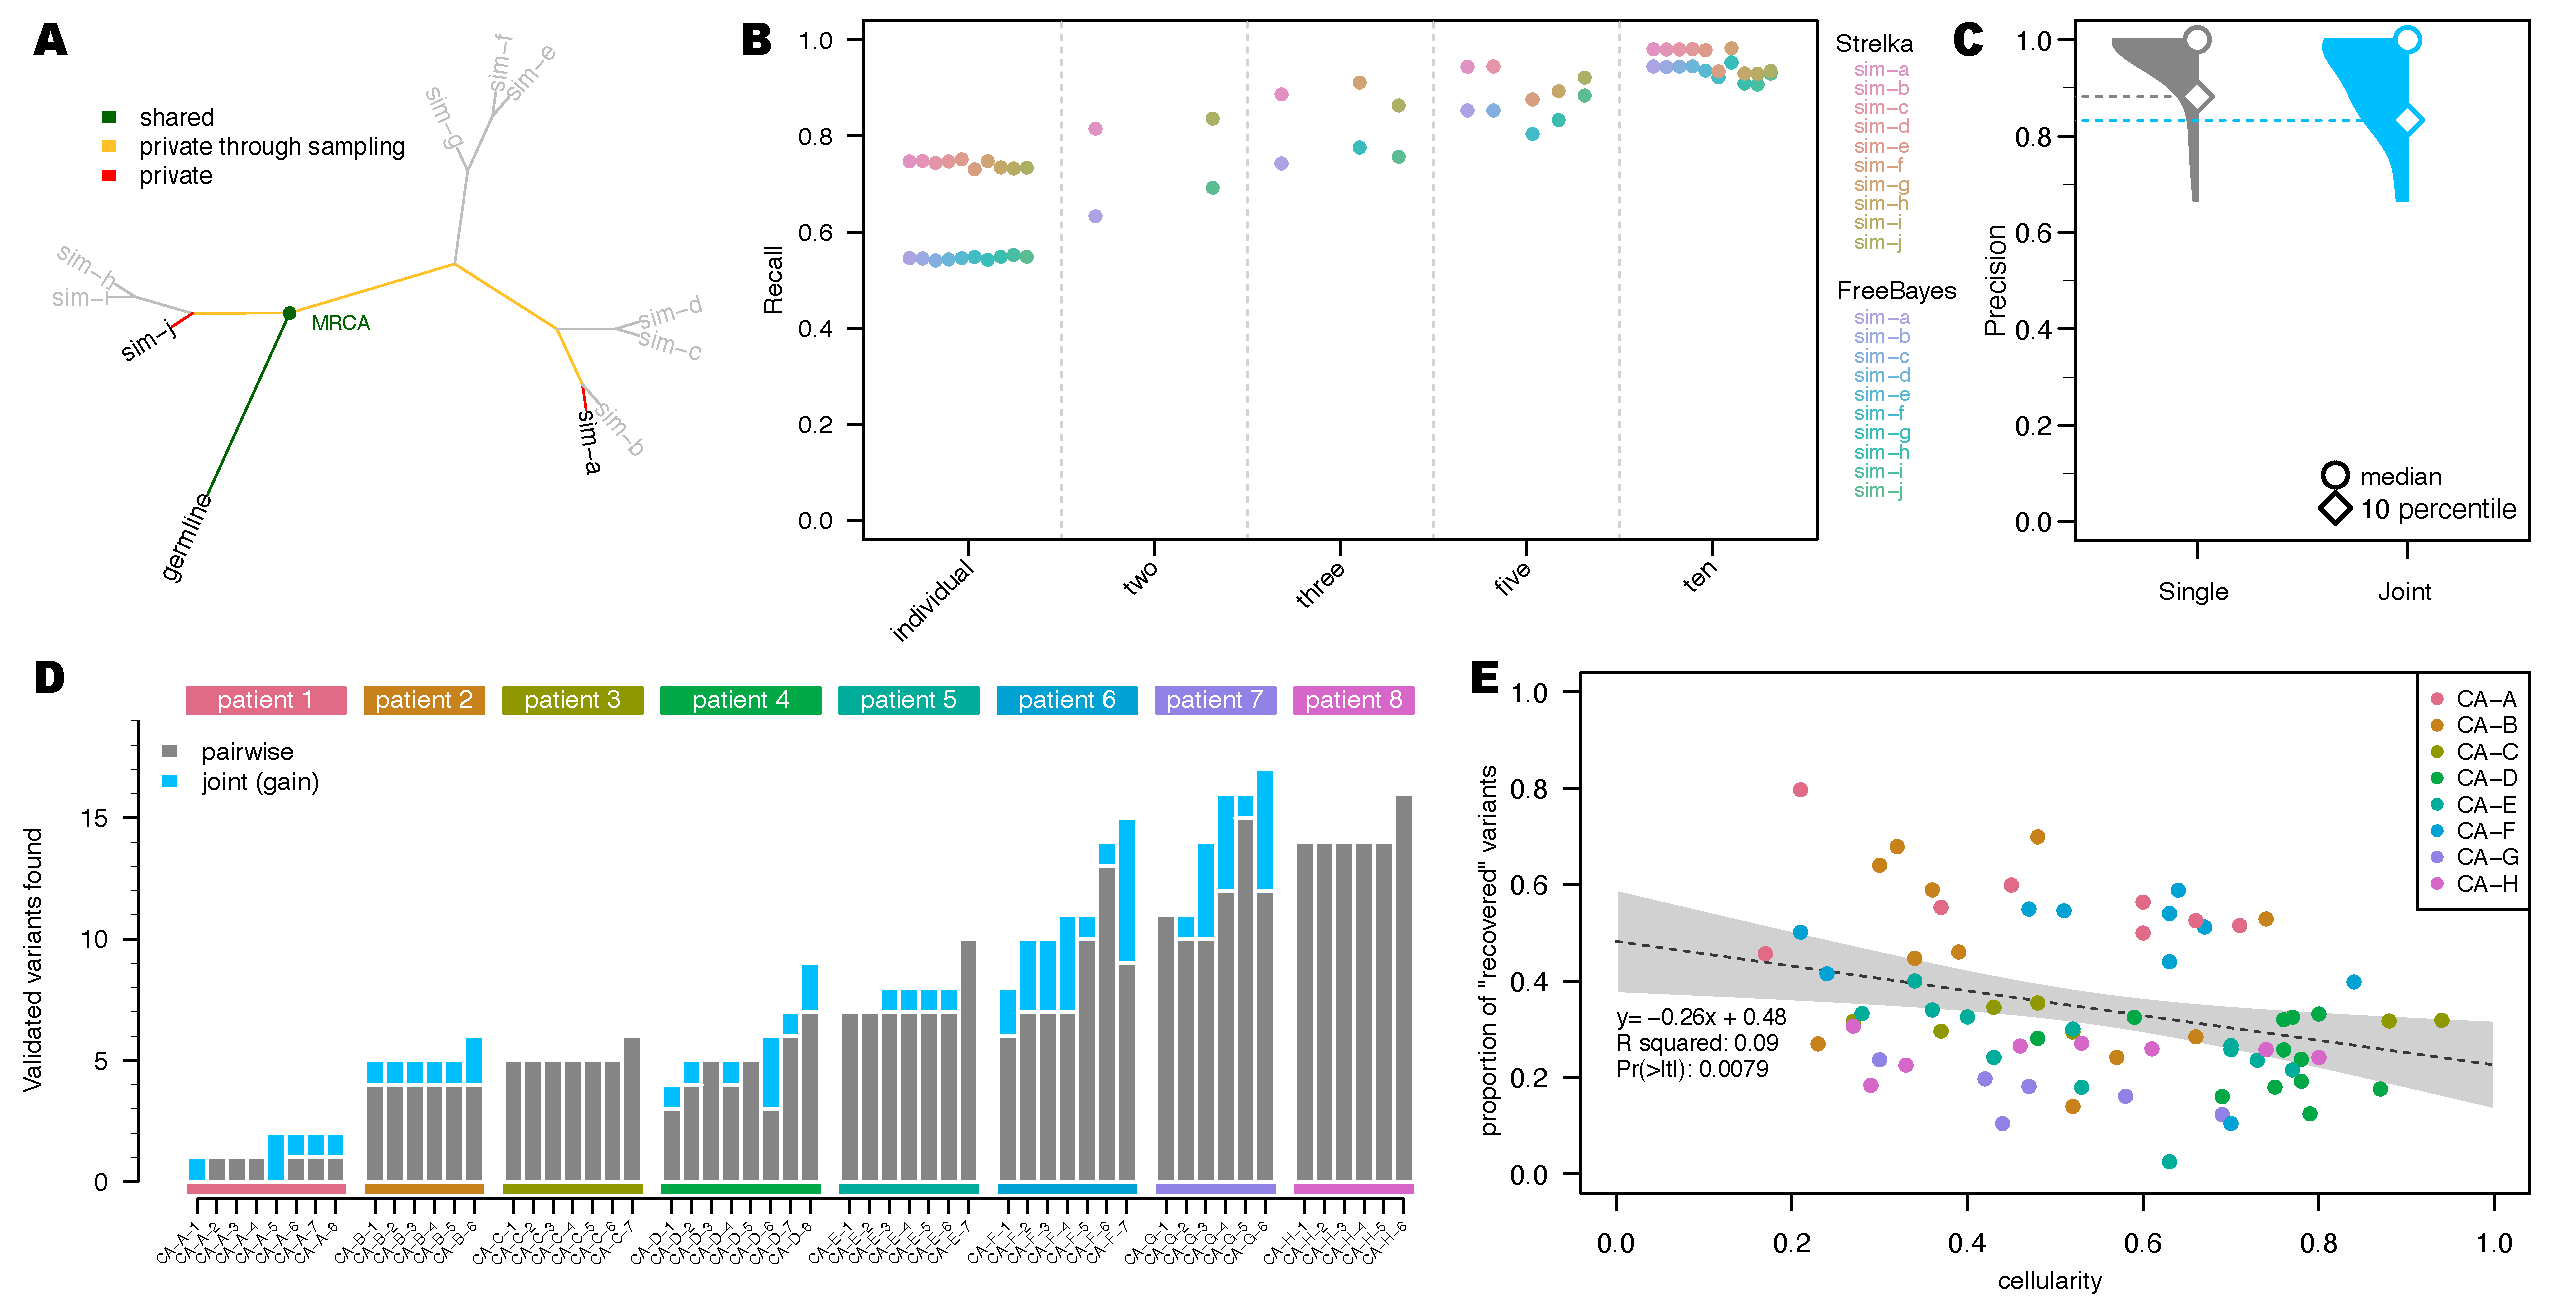
\includegraphics[width=\textwidth]{Appendices/Variantcalling/Figure_1}\vspace*{-12pt}
  \caption[Comparison of joint multi-sample and single tumour-normal paired variant calling methods]{Comparison of joint multi-sample variant calling and single tumour-normal paired calling methods; A) Simulated phylogeny highlighting two samples with high evolutionary distance (sim-a and sim-j) where MRCA denotes the most recent common ancestor. B) Recall estimates of FreeBayes and Strelka2, run in individual tumour-normal paired and joint calling configurations using two (sim-a and sim-j), three (sim-a, sim-g and sim-j), five (sim-a, sim-c, sim-f, sim-h and sim-j) and all ten tumour samples. C) Precision of Strelka2 and D) Number of variants called by Strelka2 run in both tumour-normal paired (grey) and added with joint calling configurations (blue), which have been validated by targeted amplicon sequencing (TAS). E) Correlation between cellularity and proportion of variants found only with joint calling using Strelka2Pass for clinical samples; grey area shows the "$95\%$" confidence interval for the linear model fit (dotted line).}\label{fig:varcalling:fig1}
\end{figure*}

\subsubsection{Simulated data}
\label{variantcalling-sec:simdata}
We first simulated a phylogeny with somatic and germline variants from ten tumour samples and one normal (\autoref{fig:varcalling:fig1}A and \autoref{A:fig:S01}A, B). Germline variants were simulated at a uniform allele frequency of $0.5$. Somatic VAFs were sampled from a custom distribution, modelled to favour low allele frequency variants to closely represent real world data (min VAF: $0.001$; max VAF: $1$; Fig.~S1C, D). Paired-end sequencing reads with realistic error profiles were simulated for WGS data at 160X average coverage using the ART-MountRainier software \parencite{Huang2011}. The simulated reads were aligned to GRCh38 and both germline and somatic variants from the phylogeny were spiked into the aligned reads using Bamsurgeon \parencite{Ewing2015}. We compared the workflows for FreeBayes and Strelka2 with and without our extensions for joint variant calling on the simulated datasets. The performance of Mutect2 joint variant calling was also assessed using its proposed best practice workflow. As both Mutect2 and FreeBayes do not return a verdict for each individual sample, we needed to assign each sample in the multi-sample VCF its own FILTER value. We called a somatic variant as present in a sample, if there were at least two reads supporting it for this sample and the overall FILTER showed a ``PASS``, which was the same cut-off used in the refiltering step in the Strelka2-pass workflow.

While the precision of each method without our extensions was greater than $99.8\%$, they all missed at least 25\% of all variants in the samples (i.e recall $\leq 75\%$). In contrast, the recall of the modified workflows increased to $\approx 95\%$ with only a minute decrease in the precision for both FreeBayes and Strelka2 (\autoref{A:fig:S02}). Mutect2 however, had virtually no change in precision, but the recall actually decreased from $\approx 75\%$ to $\approx 41\%$ when analysing the samples jointly (\autoref{A:fig:S02}B). Additionally, with our modified workflows, true positive variants were called with VAFs as low as 0.008 (median detected VAF $\geq 0.14$ for joint sample analysis and $\geq 0.21$ for single tumour-normal pair analysis), enabling improved distinction between true variants and technical errors (\autoref{A:fig:S03}). This improvement in performance for Strelka2 is only achieved after the refiltering step and not just a result of the second pass (\autoref{A:fig:S04}, \autoref{A:varcalling:steps}).

The performance of joint variant calling in Mutect2 was inferior compared to all other methods (\autoref{A:fig:S02}A, B). This was primarily due to the "clustered\_events" filter in Mutect2, which excluded the majority of false negative variants, with negligible contribution to the exclusion of true negative variants (\autoref{A:fig:S05}A, B). This result was unexpected as the simulated variants were evenly distributed along the genome and the corresponding allele frequencies were sampled randomly (\autoref{A:fig:S01}D).

Since the extent of the improvement in our joint calling workflows is bound by the number of shared variants between samples, we sub-sampled the simulated dataset, to show the effect of incomplete sampling on our methods, which is more likely in clinical settings. Furthermore, the evolutionary distance between the related samples in addition to the number of samples, has a major impact on the number of shared variants, as only variants acquired between the germline and the most recent common ancestor (MRCA), will benefit from the joint analysis. Therefore, we selected three sample subsets which included two, three and five samples with high evolutionary distance to show the minimum expected improvement (\autoref{fig:varcalling:fig1}A, B). There was a clear linear improvement for both FreeBayesSomatic and Strelka2Pass when increasing the number of samples even if they had a distant evolutionary relationship. In contrast, when using only two samples with a small evolutionary distance, the increase in performance was almost as large as when jointly analysing all 10 available samples. This shows that samples with a high number of shared variants will perform better in joint calling workflows (\autoref{A:fig:S06}).

\subsubsection{Clinical data}
\label{variantcalling-sec:realdata}
To validate the performance of our new workflows, we then analysed WGS and whole-exome sequencing (WES) data of multi-region tumour samples from eight patients, with multiple tumour sites (average 7 samples per patient; total number of samples 55), enrolled in a rapid autopsy program conducted at the Peter MacCallum Cancer Centre (\autoref{A:tab:S1} and \autoref{A:varcalling:clinical}) \parencite{Solomon2020, Vergara2021}. The published studies had multiple somatic variants from the clinical samples orthogonally validated through targeted amplicon sequencing (TAS). We used these TAS-validated variants as the gold standard to evaluate the performance of different workflows, acknowledging that the technical biases inherent to TAS data are different to those present in WGS and WES (\autoref{A:fig:S07}) and that there would be sampling biases depending on different tumour cells analysed in each data type.

In concordance with the results of the simulated data, our improved workflows found additional variants in all but one patient (\autoref{fig:varcalling:fig1}D, \autoref{A:fig:S08}) (total additional variants Strelka2Pass: $64$; FreeBayesSomatic: $85$) with only a slight drop in precision for FreeBayesSomatic (mean: $0.94$ vs. $0.88$) and Strelka2Pass (mean: $0.97$ vs. $0.92$). Since the panel of variants validated by TAS was limited ($7108$ bp for patients CA-B through -H), this increase in detected variants suggests that a high number of shared variants in samples are missed with current approaches, which in turn leads to an overestimation of tumour heterogeneity between samples, as these variants are thought to not be present rather than undetected.

Even though the number of shared variants is a major influencing factor when jointly calling variants, low cellularity samples benefit more from the joint calling, as conventional methods cannot reliably distinguish low allele frequency variants from noise. Through a joint analysis approach, the number of recovered variants is higher in low cellularity samples, which indicates, that especially for clinical samples with variable tumour purity, joint analysis can have a major impact on improving performance (\autoref{fig:varcalling:fig1}E, \autoref{A:fig:S09}).

Mutect2 in contrast, did not show significant improvement in any sample in its joint calling configuration, but showed inferior performance compared to the tumour-normal pairwise approach in two samples (\autoref{A:fig:S08}E), similar to its decreased performance in the simulated data (\autoref{A:fig:S02}). This was due to true variants being removed by the internal filters of the tool (\autoref{A:fig:S05}C, D). This is in stark contrast to our novel workflows, where the joint analysis preserves all called sites from the pairwise method and finds additional variants. Overall, Mutect2 found less validated variants in all patients than both Strelka2Pass (mean: $2.2$) and FreeBayesSomatic (mean: $2.5$) with comparable levels of precision (\autoref{A:fig:S08}, \autoref{A:fig:S10}) but longer run times (\autoref{A:tab:S2}).

Our improved workflow also enabled the discovery of multiallelic variants with Strelka2, which led to the discovery of on average $42$ additional variants (min: $1$; max: $535$) in the analysed WES and $987$ additional variants in the WGS (min: $81$; max $2329$). These variants are strong indicators of sub clonal structure and are invaluable for the study of evolutionary trajectories in cancer as shown in the following sections.


